\documentclass{article}
\usepackage{leonine,amsmath,amssymb,amsthm,graphicx, setspace}%%xy, setspace, amscd (commutative diagram)
\title{Notes}
\author{Eric Purdy \footnote{Department of Computer Science, University of Chicago. Email: epurdy@uchicago.edu}}

\newcommand\note[1]{\mar{#1}}
% \newcommand\note[1]{}

%% \newcommand\spk[2]{\includegraphics[width=#1mm]{images/#2.png}}
\newcommand\spk[2]{\framebox{images/#2.png}}

%%\doublespace

\begin{document}
\maketitle


\subsubsection{Deformation models (VERY ROUGH)}

\note{datapoints -> objects, throughout this section}
We are working with datapoints in a space $\XXX$. Let $\CCC$ be a
space of correspondences between two datapoints in $\XXX$.  We leave the
notion of correspondence slightly vague; it might be a partial
matching of the pieces of the two datapoints.
\note{Hard to imagine a ``piece'' of a datapoint}

We define a deformation model $\MMM: \XXX \times \CCC \times \XXX \to
\RRR^{\ge 0}$ to be a function which maps two datapoints and a
correspondence to a matching cost. $\MMM(x_1, c, x_2)$ represents the
quality of the correspondence $c$ 
\note{kill ``given that it purports to be a correspondence''} given that it purports to be a
correspondence between $x_1$ and $x_2$. We are particularly interested
in considering this to be the negative log of a (possibly
non-normalized) probability distribution.

Given a deformation model $\MMM$, we can define a nearest-neighbor
classification algorithm on $\XXX$. If we have classes $X_1,\dots,X_k$ with
training examples $\{x_{ij} \mid j\in [n] \}$ in $\XXX$, we can classify a novel
example $x_*$ as being of the class $X_i$ which minimizes 
$$\min_{j\in [n], c\in \CCC} \MMM(x_{ij}, c, x_*).$$

Our research program is then to then to automatically generalize from the
examples $\{x_{ij}\}$ using a grammatical version of $\MMM$.

\note{Intuitively c defines a parse of X2 with X1. NN only assumes
  distances, so this claim is too broad.

What parts-based models can we cite? Correspondence-based things, like
shape matching algorithms. Ball and springs model. Pedro's Pascal model.  }

\note{Pedro does not follow this whole list}
\bitem
\item Define an agglomeration operator $\oplus$ on $\XXX$ that sticks
  two datapoints together to get another. This may require enlarging
  $\XXX$.
\item Extend $\CCC$ in such a way that it respects $\oplus$: if $c_1$
  is a correspondence between $x_1$ and $y_1$, and $c_2$ is a
  correspondence between $x_2$ and $y_2$, we want there to be a
  correspondence $c_1 \oplus_\CCC c_2$ between $x_1\oplus x_2$ and
  $y_1\oplus y_2$.
\item Redefine $\MMM$ so that $\MMM( x_1\oplus y_1, c_1 \oplus_\CCC
  c_2, x_2\oplus y_2 )$ is the sum of $\MMM(x_1,c_1,y_1)$,
  $\MMM(x_2,c_2,y_2)$, and possibly some interaction term $T( (x_1,y_1), (x_2,y_2) )$

\item Define grammars over $\XXX$, such that $\oplus$ is used to stick
  together the parts of the hierarchical decomposition

\item Learn new, grammatical class models. These will be used for
  classification like so:
$$\argmin_i \min_{x\in \XXX c\in \CCC} \MMM(x, c, x_*) - \log\PP[x
    \mid G_i].$$ We will call this parsing.  As part of this, we want
  to be able to adapt whatever minimization algorithm was used by
  $\MMM$ to find the best correspondence, and use it to find the best
  parse of $x_*$.  
\eitem

Why is it important that $\oplus$ be used for the hierarchical
decomposition? It means that the minimization algorithm of the last
point will be producing a hierarchical decomposition of $x$, and thus
of $x_*$.

\subsection{L-Systems (replace with Pedro's example, maybe move to intro)}

To motivate our discussion of curve grammars, we will first give an
amusing example of such a grammar, which is inspired by L-systems. A
Lindenmayer system, or L-system, is a parallel string rewriting
system. 
\note{They are intended to be pictures! Cite Lindenmayer's famous book.}
Although they are defined on strings, it is popular to render
their output as a picture using a ``turtle language'' akin to
Logo. They are a simple and intuitive way to generate fractal
images. Since our formalisms do not match up perfectly with the usual
definition of L-systems, we will not discuss them.

We will informally discuss curve rewriting systems, where we
iteratively replace straight lines with curves composed of straight
lines. We will represent our curves like this: \spk{10}{gline}, so that
we remember which endpoint is which.

Consider the following system\footnote{generated by $A=A+A+A--$ with
  angle $60^\circ$ in Inkscape}:
$$ \spk{10}{gline} \to \spk{10}{gbump} .$$

Applying this rule a few times, we generate \spk{10}{gline}, \spk{10}{gbump},
\spk{10}{gbump2} and \spk{15}{gbump3}.

%% An L-system might represent
%% this rewrite rule as $A\to A+A+A$. Here, if we interpret the symbol
%% $A$ as ``go forward one step'' and the symbol $+$ as ``rotate 60
%% degrees to the left'', then a turtle following the directions $A+A+A$
%% would generate the curve 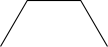
\includegraphics[width=10mm]{bump.png},
%% suitably rotated.

We now wish to construct a more complicated system. We need to start
distinguishing different kinds of curves, in this case \spk{10}{gdash}
versus \spk{10}{gline}. Consider the following system\footnote{generated by 
$A=B+A+B; B=A-B-A$ with angle $60^\circ$ in Inkscape}
\begin{align*}
\spk{15}{gline} &\to \spk{15}{gBAB} \\
\spk{15}{gdash} &\to \spk{15}{gABA}.
\end{align*}

If we start from \spk{10}{gline}, we successively generate
\spk{10}{gBAB}, \spk{20}{gsier2}, and \spk{20}{gsier3}.  Suprisingly,
after a large number of iterations, a pattern arises that may be
familiar: Sierpinski's triangle! After eight iterations, we have
(filling in the dashed lines for simplicity) curve $C$:

\spk{100}{gsier8}.

These curves were generated by Inkscape's L-system function, which has
a randomizing option. It is interesting to randomize the last
example. Here is the randomized version $C'$ I got, with fairly little
noise (10\% randomization in the length of line segments, and 5\%
randomization in the angles. These parameters only make sense in a
more standard L-system framework):

\spk{100}{gbadsier}.


\note{This is exactly the issue shape-tree addresses in contrast to other deformable models.}
This has no global similarity at all to the other curve! Inkscape is
using a Markov-like source of randomness, and little errors at the
local level add up to huge changes at the global level. If we are
going to have a statistical model for perceptual similarity of curves,
we will have to find a way to introduce long-range dependencies. This
brings us to our next section: probabilistic context-free grammars on
curves.


\subsection{Restricted Classes of Shape Grammars: ASU}

\note{ This entire section deals with the abstract portion of the
  grammar, so we are really giving restricted classes of CFG's.}

\subsubsection{Almost Single Use}

\begin{defn}
A {\em single-use grammar} is one in which every nonterminal $N\in
\NNN$ appears on the right-hand side of at most one rule, and in which
the start nonterminal(s) do not appear on the right-hand side of any rule,
and the starting form does not contain any nonterminal twice.
\end{defn}
\mar{Have to allow $L\to LL$}
\mar{appears only once on right hand side, also}
\mar{$\Pi(X)$ is set of rules with $X$ on the left hand side}

\note{Why do we care about this???}
\begin{defn}
A grammar $\GGG$ is {\em almost single-use} if $\NNN = \NNN_{NT} \cup
\NNN_{PT}$, with the following conditions:
\bitem
\item If $X\in \NNN_{NT}$, then $X$ appears at most once on the right
  hand side of at most one rule in $\RRR$, or appears at most once in
  at most one starting form in $\SSS$, but not both.
\item If $X\in \NNN_{PT}$, then $X$ appears in a rule $X\to XX$. $X$
  appears at most once on the right hand side of at most one other
  rule in $\RRR$, or at most once in at most one starting form in
  $\SSS$, but not both. Also, $X$ is on the left side of exactly two
  rules, $X\to XX$ and $X\to \ell$.
\eitem
\end{defn}

\subsection{Geometric Deformation Model, Watson}
\note{$p r q$ vs $p q r$ is confusing and probably at least one is
  wrong. Also, $p,q,r$ should have same values throughout, and it
  doesn't look like they do.} We will model the midpoint distribution
using the complex Watson distribution, defined as follows: consider
our points in $\RR^2$ as complex numbers, and let $\tilde{z} =
\left(\begin{array}{c c c} p& r& q\end{array}\right)$.  Let
  $\tilde{\mu} = \left(\begin{array}{c c c} p& \widehat{r} &
    q\end{array}\right)$, where $\widehat{r}$ is the most likely value
    of $r$. For various reasons, we will multiply $\tilde{z}$ by the
    $2\times 3$ Helmert matrix
$$H = \left(\begin{array}{c c c} 1/\sqrt{2} & -1/\sqrt{2} & 0
  \\ 1/\sqrt{6} & 1/\sqrt{6} & -2/\sqrt{6}\end{array}\right), $$ and
then normalize the result to get our coordinates:
\begin{align*}
\langle p, q, r\rangle = z &= H\tilde{z} / \|H\tilde{z}\| \\
\mu &= H\tilde{\mu} / \|H\tilde{\mu}\|
\end{align*}

Then
$$\mu_{A\to BC}(r) = Watson(\mu,\kappa) =
\frac{1}{Z(\kappa)}e^{-\kappa |z^*\mu|^2},$$ where $\kappa$ is a
concentration parameter. More details on the Watson distribution can
be found in Mardia and Dryden.

\subsection{Prior over Grammar Parameters}
\label{sec-prior-param}

\note{?? Why is this good?}

We must specify a prior for the $\mu_{X\to YZ}$ and $\rho_X$.  For
optimal results, we tailor the specific prior to the scale $s$ of the
subcurve we are modeling, where $s(C') = \frac{|C'|}{|C|}$.

Let $X\in \NNN$. Let $s$ be our scale parameter. We let
$$\rho_X \sim Dir(\alpha_1, \dots, \alpha_k),$$
where
\begin{align*}
\alpha_1 &= \alpha_{dir} e^{- \alpha_{\rho} s^2} \\
\alpha_i &= \alpha_{dir} \frac{1 - e^{- \alpha_{\rho}s^2}}{k-1}, 2\le i\le k
\end{align*}
where $\alpha_1$ corresponds to the rule $X\to \ell$.
Currently $\alpha_{dir} = 10.0$, $\alpha_\rho = 1000.0$.

Let $X\to YZ$ be a rule of $G$. Let $s$ be our scale parameter.  We
set $\mu_{X\to YZ}$ equal to a Watson distribution with random mode $\mu$ and
random concentration $\kappa$, where
$$\kappa \sim Gamma(\sigma, \theta=\bar{\kappa}/\sigma)$$
$$\mu \sim Watson(\mu_0, \alpha_{mp} \kappa)$$
where $\sigma$ is the shape parameter of the Gamma distribution, and
$\bar{\kappa} = \alpha_{\kappa} s$. 

Currently $\sigma=5$, $\alpha_\kappa = 4000.0$. $\alpha_{mp}$ is a
parameter dictating the balance between prior and observation.  We
choose $\mu_0$ to correspond with the mean of the two endpoints.


\section{Learning Parameters (change to nonparametric, so not much learning of geometry) (add EM section)}

There are two components to our model: the structure of the grammar,
and the value of the continuous parameters. If we have an appropriate
structure, learning the continuous parameters can be done using the EM
algorithm, modified so as to take priors into account.

Doing the full EM algorithm would require us to sum over all possible
parses. For the sake of simplicity and efficiency, we approximate this
by only using the parse with highest likelihood, called the Viterbi
parse.

In this section we give approximations to the maximum a posteriori
setting of the parameters given observed data. Let $C_1, \dots, C_n$
be our observed curves, $\GGG$ be our grammar (whose structure is
fixed), and let $T_i$ be the Viterbi parse tree of $C_i$ according to
$\GGG$.

\subsection{Multinomial Distribution}

We want to estimate the distribution $\rho_X$, which is distributed
according to some $Dir(\alpha_1, \dots, \alpha_m)$. For each of the
rules $X\to \lambda$, we have a count $k_i$ of how many times that
rule appears in the $T_j$. The maximum a posteriori estimate of
$\rho_X$ is then a multinomial with probabilities 
$$p_i = \frac{k_i + \alpha_i - 1}{\sum_i k_i + \sum_i \alpha_i - m}.$$

\subsection{Watson Distribution}

We wish to estimate $\mu_{X\to YZ}$, given the parses $T_1, \dots,
T_n$. For each time the rule $X\to YZ$ was used, we observe one
midpoint. Transforming these into our preferred coordinates, we get
observations $z_1, \dots, z_m$. We wish to use the $z_i$ to estimate
the parameters $\mu$ and $\kappa$ of our Watson distribution.

Let $\alpha_{mp}, \mu_0$ be defined as in Section
\ref{sec-prior-param}. Let $\gamma(\kappa;\sigma,\theta) = \log
Gamma(\kappa; \sigma,\theta)$.  Let $c(\kappa)$ be the normalizing constant
of the Watson distribution.

\begin{align*}
P(\mu, \kappa \mid z_1,\dots,z_m) &\propto
P(\mu, \kappa) P(z_1,\dots,z_m\mid \mu, \kappa) \\
&= \exp[ \alpha_{mp}\kappa \mu^* \mu_0 \mu_0^* \mu
- \log c(\alpha_{mp} \kappa) + \gamma(\kappa; \sigma,\theta)
+ \kappa \sum_i \mu^* z_i z_i^* \mu - m \log c(\kappa)
\\
&= \exp[
\kappa \mu^* (\alpha_{mp} \mu_0 \mu_0^* + \sum z_i z_i^*)\mu
- \log c(\alpha_{mp} \kappa) - m \log c(\kappa) + 
\gamma(\kappa; \sigma, \theta) ]\\
\log P(\mu, \kappa \mid z_1,\dots,z_m) &= 
c_{norm} + 
\kappa \mu^* (\alpha_{mp} \mu_0 \mu_0^* + \sum z_i z_i^*)\mu
- \log c(\alpha_{mp} \kappa) - m \log c(\kappa) + 
\gamma(\kappa; \sigma, \theta) \\
&= c_{norm} + 
\kappa \mu^* A \mu
- \log c(\alpha_{mp} \kappa) - m \log c(\kappa) + 
\gamma(\kappa; \sigma, \theta),
\end{align*}

where $A = \alpha_{mp} \mu_0 \mu_0^* + \sum z_i z_i^*$.
Since $\mu$ only appears in the term $\kappa \mu^* A \mu$,
and $A$ has non-negative eigenvalues, it is clear
that we maximize the posterior by choosing $\mu$ to be
the dominant eigenvector of $A$.
Let $\lambda_{\max}$ be the associated eigenvalue. Then

\begin{align*}
\log P(\mu, \kappa \mid z_1,\dots,z_m) &= 
c_{norm} + \kappa \lambda_{\max}(A) - 
\log c(\alpha_{mp} \kappa) - m \log c(\kappa) + 
\gamma(\kappa; \sigma, \theta)\\
\end{align*}

Taking partial derivatives, and using the approximation
$c(\kappa) = 2 \pi^2 \frac{1}{\kappa} e^\kappa$,
we arrive at the approximate solution

$$
\frac{\partial \log P(\mu, \kappa \mid, z_1,\dots,z_m)}
{\partial \kappa} = 
\lambda_{max} - \alpha_{mp} -m + \frac{1+m}{\kappa} + 
\frac{\sigma-1}{\kappa} - \frac{\sigma}{\bar{\kappa}} = 0
$$
$$
\widehat{\kappa} = \frac{\sigma+m}{\frac{\sigma}{\bar{\kappa}}
+ m + \alpha_{mp} - \lambda_{max}}
$$

$$
\widehat{\mu} = \mbox{ dominant eigenvector of }
A\mbox{, where } A = \alpha_{mp} \mu_0 \mu_0^* + \sum z_i z_i^*
$$

Examining this solution, we see that our estimate of the
midpoint is similar to the maximum likelihood estimate of
a Watson distribution, but is adapted to contain
$\alpha_{mp}$ artificial observations at the prior mode.

The posterior estimate of the concentration will be at
a maxmimum when all $z_i$ are identical and equal to 
$\mu_0$. In this case, $\lambda_{max}$ will be
$m + \alpha_{mp}$, and $\widehat{\kappa} = 
\bar{\kappa} \frac{\sigma+n}{\sigma}$. Thus, our concentration will
increase essentially linearly with the number of examples, but will never
be infinite.

In general, the $z_i$ and $\mu_0$ will be more spread out, causing $A$
to have a lower dominant eigenvalue, and lowering the concentration.

\subsubsection{Picking a Better Almost Single Use Grammar}

When constructing a grammar from a single curve, we have a choice in
how we split the curve each time. It is straightforward to do this in
such a way that we optimize the prior probability of the resulting
grammar. In practice, this means mainly choosing the midpoints to make
the subcurves straight, and the two subcurves of roughly equal length.

This is done via dynamic programming.
\mar{Explain!}

\subsubsection{Merging the Leaves}

We will usually merge all nonterminals that are ``leaves'', i.e.,
those nonterminals $N$ whose only expansions are $N\to NN, N\to \ell$.
\mar{Explain!}

\subsection{Learning a Grammar for Multiple Curves by Greedy Optimization (kill)}

It is a well-defined question to ask for the shape grammar structure
and parameters which give us the maximum posterior for a set of
training examples given our chosen prior and likelihood
models. Unfortunately, we do not know how to optimize over all grammar
structures, and we do not know how to optimize over even restricted
classes of grammars efficiently. Here we describe a restricted class
of grammars and a greedy approach to finding a reasonable structure.

\subsubsection{Incremental Incorporation}

Suppose that we have a grammar $G_n$ which is an acceptable
explanation of example curves $C_1,\dots, C_n$.  Among the restricted
class of grammars we are examining, we wish to pick the best grammar
$G_{n+1}$ to explain $C_1,\dots, C_{n+1}$. To make the problem more
tractable, we will use the Viterbi approximation, and we will only
look at $G_{n+1}$ which contain all nonterminals and rules of $G_n$.

Because of the greedy search strategy, it seems sensible
to choose our next curve $C_{n+1}$ to be the next unexplained
curve which is least likely under $G_n$. Hopefully, this will
allow us to discover all the necessary structure quickly.

We simplify matters by only considering single-use grammars.

\begin{defn}
For a curvilinear form $\Phi = \phi_1 \cdots \phi_k$, and a
closed-curve grammar $G = (\NNN,\Pi,S,T,\ell)$, let $$SUB_G(\Phi) = \{
r_1(\phi_1) \cdots r_k (\phi_k),\mid r_i \in \Pi(\phi_i) \}.$$ A derivation is
a list of curvilinear forms $\Phi_1,\dots, \Phi_k$, where $\Phi_1 =
ST$, $\Phi_k = \ell^n$, and $\Phi_{i+1} \in SUB_G(\Phi_i)$ for $1\le i
< k$.
\end{defn}

\begin{lem}
Any derivation from a single-use grammar $G$ uses each nonterminal at
most once. 
\end{lem}
\begin{proof}
Let $D = (\Phi_1, \dots, \Phi_k)$ be a derivation from $G$.  Suppose
that $\Phi_h$ and $\Phi_{h'}$ contain the same symbol $N$, where $h$
is minimal. $N$ appears on the right hand side of only one rule,
without loss of generality $r : X \to N Z$. Then, if $h>1$, $X$ must
occur in both $\Phi_{h-1}$ and $\Phi_{h'-1}$, contradicting the
minimality of $h$. If $h=1$, $N$ is one of the start nonterminals, so
$G$ should not have such a rule $r$.

Suppose that $\Phi_h$ contains some nonterminal $N$ twice, where $h$
is minimal. Then, if $h>1$, we can again find the unique $r : X \to N
Z$ with $N$ on the right-hand side. Then $X$ must appear twice in
$\Phi_{h-1}$, contradicting the minimality of $h$. If $h=1$, then the
starting form of $G$ contains a repeated nonterminal, which is not
allowed.
\end{proof}

\subsubsection{What Grammars are We Searching Over?}

\subsubsection{Incremental Incorporation Formula}

We wish to maximize 
\begin{align*}
\frac{P(\GGG \mid C_1, \dots, C_n, C)}{P(\GGG_n\mid C_1, \dots, C_n)}
&= \frac{P(\GGG)}{P(\GGG_n)} \cdot 
\frac{P(C_1,\dots,C_n, C\mid \GGG)}{P(C_1,\dots,C_n \mid \GGG_n)}
\end{align*}

Focusing on the first factor, the prior, we can write
\begin{align*}
\frac{P(\GGG)}{P(\GGG_n)} &=
\frac{P_{struct}(\GGG)}{P_{struct}(\GGG_n)}
\cdot
\frac{P(\MMM)}{P(\MMM_n)}
\cdot
\frac{P(\XXX)}{P(\XXX_n)} \\
&= 
\frac{P_{struct}(\GGG)}{P_{struct}(\GGG_n)}
\cdot
\prod_{\mu_{X\to YZ}\in \MMM\sm \MMM_n} P(\mu_{X\to YZ})
\cdot
\prod_{\rho'_X \in \XXX \sm \XXX_n} P(\rho'_X)
\cdot 
\prod_{\rho_X \in \XXX_n} \frac{P(\rho'_X)}{P(\rho_X)},\\
\end{align*}
assuming that we do not change the existing midpoint distributions.

We can approximate $P_{struct}(\GGG)/P_{struct}(\GGG_n)$ in a nice
way. Recall that $P_{struct}(\GGG) = \frac{1}{Z} e^{-|enc(\GGG)|}$, so
that $P_{struct}(\GGG)/P_{struct}(\GGG_n) = e^{ |enc(\GGG_n)| -
  |enc(\GGG)|}$. Thus
\begin{align*}
-\log\left(\frac{P_{struct}(\GGG)}{P_{struct}(\GGG_n)}\right) &=
\log |\NNN| + (3 \log |\NNN| + 1)|\RRR| + (\log|\NNN|| + 1)|\NNN| \\ 
&\quad - \log |\NNN_n| + (3 \log |\NNN_n| + 1)|\RRR_n| + (\log|\NNN_n|| + 1)|\NNN_n|. \\ 
\intertext{Making the reasonable approximation that
$\log|\NNN| \approx \log |\NNN_n|$,}
&\approx (3 \log |\NNN_n| + 1)[|\RRR \sm \RRR_n|] + 
(\log|\NNN_n|| + 1) [|\NNN \sm \NNN_n|]. \\ 
\end{align*}
We can thus keep track of this change by charging $\log|\NNN_n|+1$ to
introduce a new nonterminal, and $3\log|\NNN_n|+1$ to introduce a new
binary rule.

We now turn our attention to the second overall factor, the
likelihood.  Using the Viterbi approximation, we can write
\begin{align*}
\frac{P(C_1,\dots,C_n, C\mid \GGG)}{P(C_1,\dots,C_n \mid \GGG_n)}
& \approx
\frac{P(C_1,\dots,C_n \mid T_1,\dots, T_n, \GGG)}{P(C_1,\dots,C_n \mid T_1,\dots, T_n, \GGG_n)}
\cdot
\frac{P(T_1,\dots,T_n \mid  \GGG)}{P(T_1,\dots,T_n \mid  \GGG_n)} \\
& 
\cdot
P(C\mid T, \GGG)
\cdot
P(T\mid \GGG)
\end{align*}
Since we are fixing the parameters of $\MMM_n$, the first factor is
one. The second factor is $\prod_{X\to \lambda\in \RRR_n}
\frac{\rho'_X(\lambda)^{\#(X\to \lambda)}}{\rho_X(\lambda)^{\#(X\to
    \lambda)}}$.

Sticking everything together, and using the formulas for $P(C\mid T,
\GGG), P(T\mid \GGG)$, we wish to minimize

\begin{align*}
-\log\left(
\frac{P(\GGG \mid C_1, \dots, C_n, C)}{P(\GGG_n\mid C_1, \dots, C_n)}
\right) 
\approx&
(3 \log |\NNN_n| + 1)[|\RRR \sm \RRR_n|] + 
(\log|\NNN_n|| + 1) [|\NNN \sm \NNN_n|] + \\
& \sum_{\mu_{X\to YZ}\in \MMM\sm \MMM_n} -\log P(\mu_{X\to YZ}) +\\
& \sum_{\rho'_X\in \XXX \sm \XXX_n} -\log P(\rho'_X) +\\
& \sum_{\rho_X \in \XXX_n} \left(\log P(\rho_X) -\log P(\rho'_X)\right) + \\
& \sum_{[X\to \lambda]\in \RRR_n} \#(X\to \lambda\text{ in } T_1,\dots,T_n)
\left( \log \rho_X(\lambda) - \log \rho'_X(\lambda) \right) \\
& \sum_{[X\to YZ]_{pqr}\in R(T)} -\log \mu_{X\to YZ}(p,q,r) \\
& \sum_{X_{c_i c_j}\in V_{NT}} -\log\rho'_{X}(rhs(X_{c_i c_j}))
\end{align*}

Since we can derive the optimal $\GGG$ from $\GGG_n$ and the parse
tree $T$, we need only search over $T$. We can optimize this quantity
by dynamic programming, by charging every term in this formula to some
node of $T$. Specifically, for $X_{c_i c_j}\in V_{NT}$, we charge
\bitem
\item $(4\log |\NNN_n| +2) - \log P(\mu_{X\to YZ}) - \log P(\rho'_X)
  -\log \mu_{X\to YZ}(c_i,c_k,c_j) - \log \rho'_X(YZ)$ if $X$ is a new,
  non-preterminal symbol, where $Y_{c_i c_k}, Z_{c_k c_j}$ are the
  children of $X_{c_i c_j}$
\item $(4\log |\NNN_n| +2) - \log P(\mu_{X\to XX}) - \log P(\rho'_X)
  -\log \mu_{X\to XX}(c_i,c_k,c_j) - \log \rho'_X(XX)$ if $X$ is a new
  pre-terminal symbol, and we are at the root of $X$'s subtree
\item $-\log \mu_{X\to XX}(c_i,c_k,c_j) - \log \rho'_X(XX)$ if $X$ is a new
  pre-terminal symbol, and we are NOT at the root of $X$'s subtree
\item $\log P(\rho_X) - \log P(\rho'_X) + \sum_{[X\to \lambda]\in
  \RRR_n} \#(X\to \lambda \text{ in } T_1,\dots, T_n) (\log
  \rho_X(\lambda) - \log \rho'_X(\lambda)) -\log_{\mu_{X\to YZ}} (c_i,
  c_k, c_j) - \log \rho'_X(YZ)$ if $X$ is an old nonterminal, but
  $Y,Z$ are new nonterminals, where $Y_{c_i c_k}, Z_{c_k c_j}$ are the
  children of $X_{c_i c_j}$
  \mar{also $3 \log|\NNN_n| + 1$ for new rule description}
\item $ -\log_{\mu_{X\to YZ}} (c_i, c_k, c_j) - \log \rho'_X(YZ)$ if
  $X,Y,Z$ are all old nonterminals
\item $ - \log \rho_X(YZ)$ if
  $X$ is an old nonterminal, and $\ell_{c_i c_j}$ is the child of
  $X_{c_i c_j}$
\item $ - \log \rho'_X(YZ)$ if
  $X$ is a new nonterminal, and $\ell_{c_i c_j}$ is the child of
  $X_{c_i c_j}$
\eitem


\subsubsection{Multinomial penalty notes}

Also, for every use of $X$ in parsing $C_1, \dots, C_n$, the
probability of $X\to \lambda$ for $\lambda \ne YZ$ is slightly lower
than before.

We make the simplifying assumption that curves already processed will
receive the same parse as before. This makes the updated maximum a
posteriori probabilities straightforward to compute from the prior
distribution and the existing counts.
  
Let $X$ be a nonterminal with $r$ rules, with usage counts $k_1, \dots,
k_r$.

Let $N = k_1 + ... + k_r$.  Let $k_{r+1} = 1$.  Let $\alpha_1, \dots,
\alpha_{r+1}$ be the parameters of the Dirichlet prior on $r$ rules,
and $\beta_1, \dots, \beta_{r+1}$ be the parameters of the Dirichlet
prior on $r+1$ rules. Let $A = \sum_i \alpha_i, B = \sum \beta_i$.

Let
$$p_i =  (k_i + \alpha_i -1) / ( N + A -r) \mbox{ for } i=1..r$$
$$q_i = (k_i + \beta_i -1) / ( N+1 + B -(r+1)) \mbox{ for } i=1..r+1.$$
These are the MAP estimates of the parameters. 

Then the cost of making the change (the negative log ratio) is
$$\log \left[ Dir(p_1,...p_r; \alpha_1,...,\alpha_r) /
Dir(q_1,...,q_{r+1}; \beta_1,...,\beta_{r+1}) \right] +
\sum_{i=1}^r k_i \log(p_i) - \sum_{i=1}^{r+1} k_i \log(q_i).$$

This cost depends only on the identity of $X$, so we can compute it
beforehand in a straightforward way.

\subsection{Open Questions}

\subsubsection{Almost Single Use Grammars}

\mar{orphaned: We are searching over this space, while requiring that
  $X\to XX$ rules have a flat midpoint.}

\begin{lem}
Let $\GGG$ be an almost single-use grammar, $C$ a curve, and $T$ a
parse tree. Then, if $X\in \NNN_{NT}$, there is at most one $X_{pq}$
in $V$. If $X\in \NNN_{PT}$, then vertices of the form $X_{pq}$ form a
single subtree of $T$.
\end{lem}
\begin{proof}
First part is same as before.

Second part: Since $X\to XX$ and $X\to \ell$ are the only
substitutions for $X$, it is clear that all descendants of $X_{pq}$
will be either $X_{p'q'}$ or $\ell$. Thus, we need only prove that
there is at most one such subtree. Consider the set of $X_{pq}$ whose
parent is not of the form $X_{p'q'}$, and suppose that there are at
least two. Recall that $X$ appears on the right hand side of only two
rules, $X\to XX$ and $Z\to XY$. Furthermore, $Z\notin \NNN_{PT}$, since
$Z\to XY$ is not of the form $Z\to ZZ$. Thus, we will have two
occurrences of $Z$, but $Z\notin \NNN_{PT}$, and the first part of the
lemma is violated for $Z$.
\end{proof}


%% The parse of $C_{n+1}$ under $G_{n+1}$ will be a parse tree labeled
%% with nonterminals from $\NNN_n$ and some new nonterminals. Since our
%% new grammar must be single-use, and assuming that it has no unused
%% nonterminals, each new nonterminal will parse exactly one subcurve of
%% $C_{n+1}$. We need only consider adding nonterminals in
%% $\NNN_{C_{n+1}} = \{N_C \mid C \subseteq C_{n+1}\}$, and rules in
%% $\Pi_{C_{n+1}} = \{r_{C, C'} : N_{CC'} \to N_C N_{C'}\mid C,C'
%% \subseteq C_{n+1}\}$ and $\Pi_{C_{n+1},G} = \{r_{N,C,C'} : N \to N_C
%% N_{C'} \mid N\in \NNN_n, C,C'\subseteq C_{n+1}\}$. Since our grammar
%% is single-use, we will add only one of $r_{C,C'}, r_{N,C,C'}$. 

%% In order to make our grammar able to use either of these rules, we
%% must add enough rules to transform both $N_C$ and $N_{C'}$ into
%% $\ell^k$ for some $k$. The optimal grammar will only add rules used in
%% the Viterbi parse of $C_{n+1}$, so it will have new rules
%% $r_{N_1,D_1,D'_1}, \dots, r_{N_k, D_k, D'_k}$ for some disjoint
%% subcurves $D_1, D'_1, \dots, D_k, D'_k$, and it will have rules
%% $r_{C,C'}$ decomposing each $D_i$ and $D'_i$ down to single segments.

%% There is an issue here - is the new Viterbi parse constrained to be
%% consistent with the old Viterbi parse? Ideally, the answer would be
%% no...

%% We can (approximately) calculate the effect of each of these additions
%% on the posterior in isolation. There are four sources of change:


\end{document}
